\chapter{Desviación estándar de una función de varias variables}\label{sec:propdesv}

Supongamos que la magnitud del valor que queremos hallar, depende de las variables $x^1, x^2, \dots, x^m$  mediante la relaci'on funcional $y=f(x^\alpha)$, $\alpha=1,\dots,m$. Luego de realizar $N$ medidas para cada una de las $m$ variables, tenemos
\begin{center}
\begin{tabular}{cccccc}
%\hline 
$x^1_1$ & $x^1_2$ & $\cdots$ & $x^1_N$ & ; & $\bar{x}^1$ \\ 
%\hline 
$x^2_1$ & $x^2_2$ & $\cdots$ & $x^2_N$ & ; & $\bar{x}^2$ \\ 
%\hline 
$\vdots$ & $\vdots$ & $\vdots$ & $\vdots$ & ; & $\vdots$ \\ 
%\hline 
$x^m_1$ & $x^m_2$ & $\cdots$ & $x^m_N$ & ; & $\bar{x}^m$.
%\hline 
\end{tabular} 
\end{center}
Escribimos las desviaciones respecto al promedio como $\Delta x^1_i, \Delta x^2_i, \cdots \Delta x^m_i$, donde
\begin{equation}
\Delta x^1_i:=x_i^1-\bar{x}^1, \qquad \Delta x^2_i:=x_i^2-\bar{x}^2,
\end{equation}
etc.

Las magnitudes determinadas indirectamente, estarán dadas por cada uno de los conjuntos de medidas mediante la relaci'on funcional:
\begin{align}
y_1 &= f(x^1_1,x^2_1,\cdots, x^m_1), \\
\vdots &= \quad\vdots  \\
y_i &= f(x^1_i,x^2_i,\cdots, x^m_i),\\
\vdots &= \quad \vdots,  \\
y_N &= f(x^1_N,x^2_N,\cdots, x^m_N).
\end{align}

Desarrollando en serie de Taylor a primer orden en torno de los valores medios, podemos escribir:
\begin{align}
y_i & = f(x^1_i,x^2_i,\cdots, x^m_i)\\
&\approx  f(\bar{x}^1,\bar{x}^2,\cdots, \bar{x}^m)+ \sum_{\alpha=1}^m\left.\frac{\partial f}{\partial x^\alpha}\right|_{\bar{x}^\alpha}(\Delta x^\alpha_i).
\end{align}

Las diferencias respecto al valor de la función evaluada en el promedio de cada conjunto de mediciones se pueden expresar como
\begin{align}
\Delta y_i &:= y_i-f(\bar{x}^1,\cdots, \bar{x}^m)\\
&\approx  \sum_{\alpha=1}^m\left.\frac{\partial f}{\partial x^\alpha}\right|_{\bar{x}^\alpha}(\Delta x^\alpha_i).
\end{align}

Calculamos con esto la varianza (el cuadrado de la desviaci'on est'andar) de $y$:
\begin{align}
\sigma_y^2 &:= \sum_{i=1}^N\frac{1}{N-1}(\Delta y_i)^2 \\
&\approx \frac{1}{N-1}\left[\sum_{i=1}^N\left[\left(\left.\frac{\partial f}{\partial x^1}\right|_{\bar{x}}\right)^2 (\Delta x^1_i)^2 +\cdots + \left(\left.\frac{\partial f}{\partial x^m}\right|_{\bar{x}}\right)^2(\Delta x^m_i)^2 \right.\right. \nonumber \\
& \quad +  2\left(\left.\frac{\partial f}{\partial x^1}\right|_{\bar{x}}\right)\left(\left.\frac{\partial f}{\partial x^2}\right|_{\bar{x}}\right)(\Delta x^1_i)(\Delta x^2_i)+\cdots \nonumber\\
& \quad \left.\left.  +2\left(\left.\frac{\partial f}{\partial x^{m-1}}\right|_{\bar{x}}\right) \left(\left.\frac{\partial f}{\partial x^m}\right|_{\bar{x}}\right)(\Delta x^{m-1}_i)(\Delta x^m)\right]\right],
\end{align}
donde $\bar{x}=(\bar{x}^1,\cdots, \bar{x}^m)$.

Separamos esta 'ultima expresi'on en dos casos. 

\begin{itemize}
\item Caso 1. Cuando las variables medidas est'an correlacionadas.
Para este caso, la desviación estándar de los valores de $y$ est'a dada por la raíz cuadrada de la expresi'on que se obtuvo.

\item Caso 2. Cuando las variables medidas no están correlacionadas.
En este caso, la suma de todos los t'erminos cruzados son cero (o despreciable!), por lo que la expresi'on se reduce a
\begin{equation}
\sigma_y^2 \approx \frac{1}{N-1}\sum_{i=1}^N\left[\left(\left.\frac{\partial f}{\partial x^1}\right|_{\bar{x}}\right)^2 (\Delta x^1_i)^2 +\cdots + \left(\left.\frac{\partial f}{\partial x^m}\right|_{\bar{x}}\right)^2(\Delta x^m_i)^2\right]
\end{equation}
\end{itemize}

Una manera muy simple de visualizar que los t'erminos cruzados no contribuyen al valor de $\sigma_y^2$, consiste en observar la figura \ref{fig-dist}, donde en cada eje se grafic'o una variable distinta. Las dos im'agenes superiores, de la misma figura, son casos sin correlaci'on entre las variables medidas y las dos figuras inferiores tienen una clara correlaci'on. 
Luego, dividimos cada una de estas figuras en 4 cuadrantes. En todas las figuras el t'ermino cruzado $\sum_i(x_i^\alpha-\bar{x}^\alpha)(x_i^\beta-\bar{x}^\beta)$ (con $\alpha\neq\beta$) es positivo en los cuadrantes I y III y negativo en los cuadrantes II y IV. 
Para las dos figuras superiores, el n'umero de medidas en cada uno de los cuadrantes son iguales, por lo que la suma total de los cuatro cuadrantes ser'a igual a cero. 
Para las dos figuras inferiores, se ve claramente una correlaci'on, es decir, si una de las variables crece la otra tiene una tendencia definida, dejando en evidencia que si hay dependencia entre estas y al dividir en 4 cuadrantes el n'umero de medidas en los cuadrantes I y III no son iguales a las medidas de los cuadrantes II y IV, tal que la suma total no es cero. 

La varianza de $\sigma_y^2$ de $y$ puede entonces relacionarse con la varianza $\sigma_\alpha$ de cada varible independiente $x_\alpha$ por medio de la expresión
\begin{equation}\label{pe}
\sigma_y^2\approx\sum_{\alpha=1}^m\left(\left.\frac{\partial f}{\partial x^\alpha}\right|_{\bar{x}}\right)^2\sigma_\alpha^2.
\end{equation}

\begin{figure}[h!]
\begin{center}
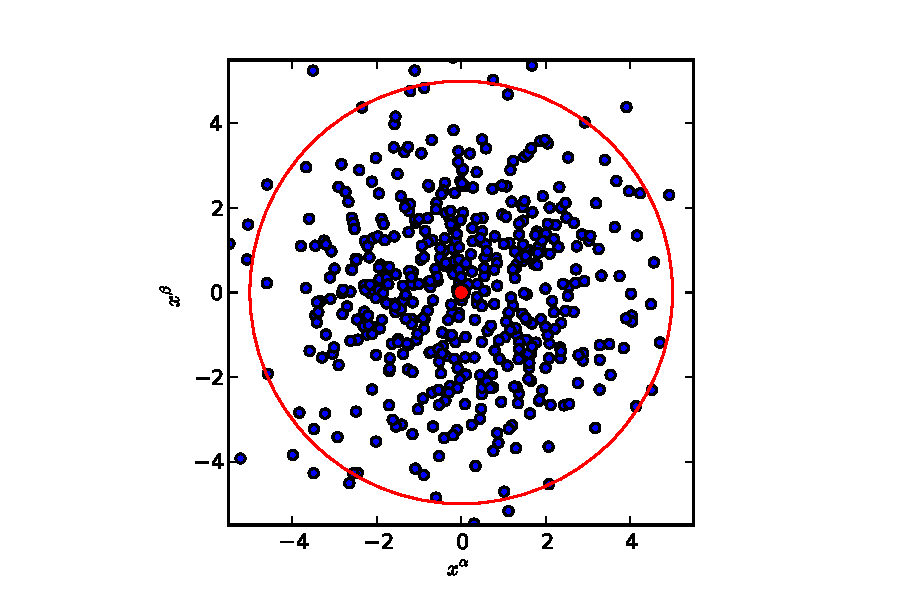
\includegraphics[width=7cm]{figs/fig-1x1.pdf}  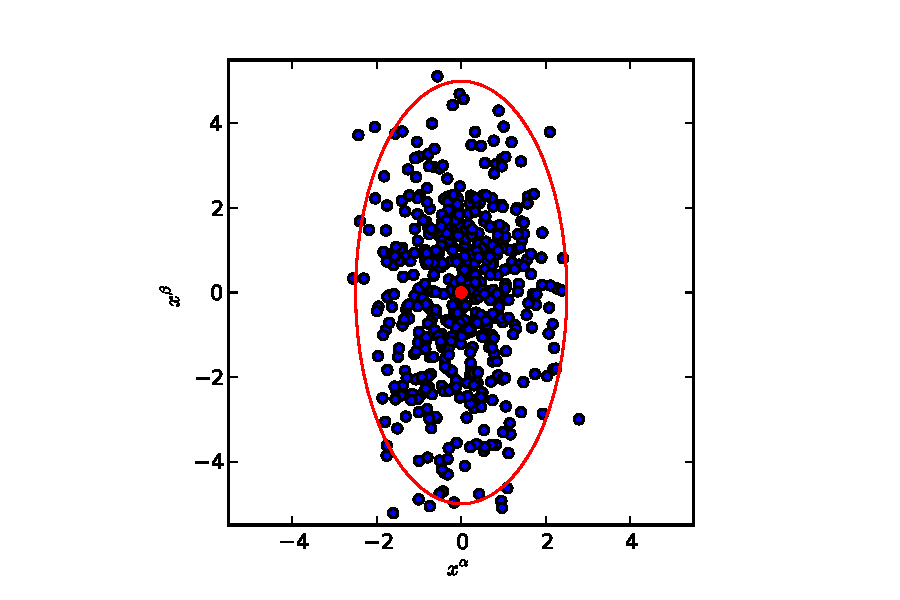
\includegraphics[width=7cm]{figs/fig-1x2.pdf}
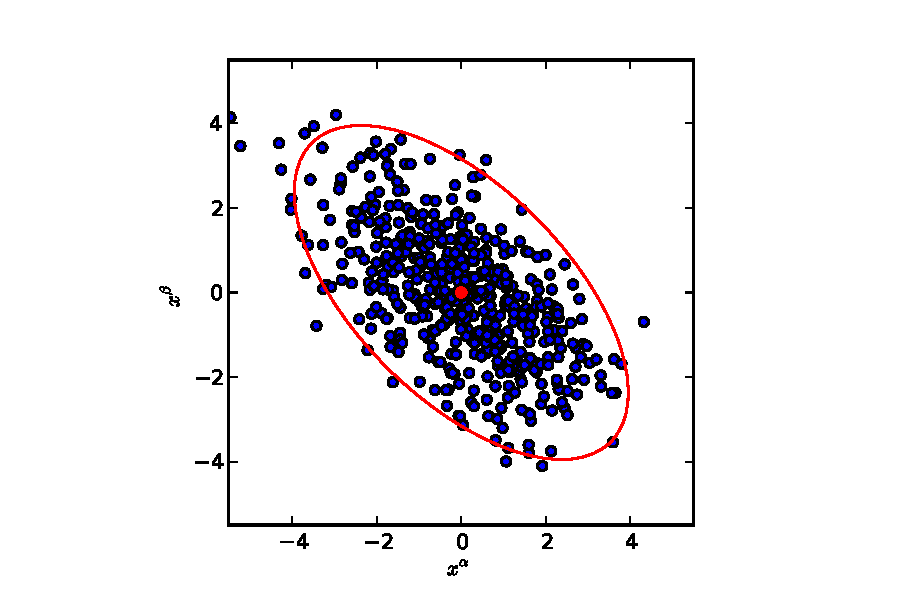
\includegraphics[width=7cm]{figs/fig-1x2rot1.pdf}  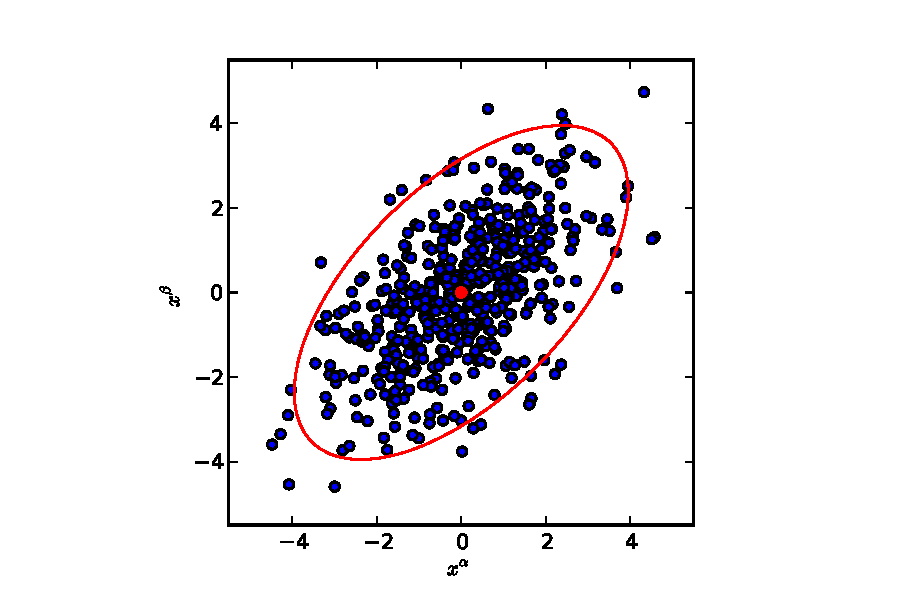
\includegraphics[width=7cm]{figs/fig-1x2rot2.pdf}
\caption{Distribuciones normales bivariadas.}
\end{center}
\label{fig-dist}
\end{figure}

\section{Error en la determinación de parámetros usando MMC}

Para encontrar la incerteza en la estimación de los parámetros $b_0$ y $b_1$ determinados por el MMC ponderado podemos usar el resultado de la sección \ref{sec:propdesv}. Cada punto de nuestros datos, caracterizados por el par $(x_i,y_i$) determina, junto con los errores $\Delta y_i$ determinan los valores de el coeficiente de posición $b_0$ y la pendiente $b_1$ a través de las expresiones \ref{b0MMCP} y \ref{b1MMCP}. Por lo tanto, podemos considerar a $b_0$ como una función particular de las $N$ `variables' $y_i$, donde cada uno de estos valores tiene un error $\Delta y_i$ (estamos ignorando el posible error de $x_i$). Si cada uno de los errores $\Delta y_i$ es la desviación estándar de muchos valores medidos para un correspondiente valor de $x_i$ dado ($\Delta y_i=\sigma_i$), entonces podemos aplicar \ref{pe} para calcular la desviación estándar de $b_0$, usando
\begin{equation}
\sigma_{b_0}^2\approx\sum_{i=1}^N\left(\frac{\partial b_0}{\partial y_i}\right)^2\sigma_i^2.
\end{equation}
A partir de \ref{b0MMCP} encontramos
\begin{equation}
\frac{\partial b_0}{\partial y_i}=\frac{1}{\Delta}\left(\frac{1}{\sigma_i^2}\sum_j\frac{x_j^2}{\sigma_j^2}-\frac{x_i}{\sigma_i^2}\sum_j\frac{x_j}{\sigma_j^2}\right)
\end{equation}
\begin{equation}
\Delta:=\left(\sum_i\frac{1}{\sigma_i^2}\right)\left(\sum_j\frac{x_j^2}{\sigma_j^2}\right)-\left(\sum_i\frac{x_i}{\sigma_i^2}\right)^2.
\end{equation}
Con esto, luego de algo de álgebra, obtenemos
\begin{equation}
\sigma_{b_0}^2\approx \frac{1}{\Delta}\sum_i\frac{x_i^2}{\sigma_i^2}.
\end{equation}
Análogamente, para la pendiente $b_1$, se encuentra
\begin{equation}
\sigma_{b_1}^2\approx \frac{1}{\Delta}\sum_i\frac{1}{\sigma_i^2}.
\end{equation}
Note que en el caso particular en que todos los errores $\sigma_i$ son iguales ($\sigma_i=\sigma$) el MMC ponderado suministra los mismos valores para los coeficientes ajustados, y además
\begin{equation}
\sigma_{b_0}^2\approx \frac{\sigma^2\left(\sum_i x_i^2\right)}{N\left(\sum_i x_i^2\right)-\left(\sum_i x_i\right)^2},
\end{equation}
\begin{equation}
\sigma_{b_1}^2\approx \frac{\sigma^2N}{N\left(\sum_i x_i^2\right)-\left(\sum_i x_i\right)^2}
\end{equation}.
%\paragraph{Ejemplo:}
%Calculemos el 'area de un tri'angulo midiendo diferentes lados y diferentes alturas. Supongamos que disponemos de una regla graduada en mil'imetros y que los diferentes lados y sus correspondientes alturas est'an dadas por: 
%\begin{align}
%a &= (16,09\pm 0,02)\text{ cm}, \qquad h_a= (10,66\pm 0,03)\text{ cm}, \\
%b &= (10,81\pm 0,02)\text{ cm}, \qquad h_b= (15,84\pm 0,03)\text{ cm}, \\
%c &= (17,78\pm 0,02)\text{ cm}, \qquad h_c= (9,66\pm 0,03)\text{ cm}.
%\end{align}
%Para calcular el 'area del tri'angulo rect'angulo debemos utilizar la expresi'on:
%\begin{equation}
%S=\frac{\text{base}\times\text{altura}}{2}.
%\end{equation}
%En general la podemos escribir de la siguiente forma:
%\begin{align}
%S &= \frac{(b\pm\Delta b)(b\pm\Delta b)}{2}=\frac{bh\pm (h\Delta b+b\Delta h)}{2}, \\
%S_a &= (85,7597\pm 0,3478)\text{ cm}^2 \quad \Rightarrow\quad S_a= (85,8\pm 0,4)\text{ cm}^2, \\
%S_b &= (85,6152\pm 0,345)\text{ cm}^2 \quad \Rightarrow\quad S_b= (85,6\pm 0,4)\text{ cm}^2, \\
%S_c &= (85,8774\pm 0,3227)\text{ cm}^2 \quad \Rightarrow\quad S_c= (85,9\pm 0,4)\text{ cm}^2.
%\end{align}
%Los valores son iguales dentro de las imprecisiones experimentales.
%?`Qu'e valor representa mejor el 'area del tri'angulo?
%
%Utilizamos el promedio aritm'etico para encontrar el valor m'as probable
%\begin{align}
%S &= \bar{S}\pm\Delta S, \\
%\bar{S} &=\frac{1}{N}\sum_{i=1}^N S_i=\frac{1}{3}\sum_{i=1}^N S_i=85,8, \\
%\Delta S &= \sqrt{\frac{1}{N}\sum_{i=1}^N (S_i-\bar{S})^2}=\sqrt{\frac{1}{3}\left(0^2+0,2^2+0,1^2\right)}=0,2.
%\end{align}
%Finalmente el resultado queda expresado como:
%\begin{equation}
%\bar{S}=(85,8\pm 0,4)\text{ cm}^2,
%\end{equation}
%donde $0,4$ es el mayor entre el error cuadr'atico medio y la propagaci'on del error asociado a cada 'area. 
%
%
%
%
%
%
%
%Para el caso en que se mida varias veces la misma cantidad y suponiendo
%que los errores asociados a estas medidas se producen por causas
%aleatorias, un buen estimador del error o de la variabilidad del resultado, podría ser la desviación estándar; expresando el resultado de nuestro experimento como
%\begin{equation}
%\bar{x}\pm \Delta x,
%\end{equation}
%donde $\bar{x}$ es el \textbf{promedio} de nuestras medidas y $\Delta x$ es el
%mayor error, entre el error asociado al instrumento y el error
%calculado:
%
%\begin{equation}
%\bar{x}:=\frac{1}{N}\sum_{i=1}^N x_i\qquad \text{(promedio).}
%\end{equation}
%
%\begin{equation}
%s:=\sqrt{\frac{1}{(N-1)}\sum_{i=1}^N(x_i-\bar{x})^2}, \qquad \text{(desviación estándar).}
%\end{equation} 
%
%En este punto es bueno tener presente que existen otros valores medios y otras estimaciones para el error, como:
%\begin{equation}
%x_g:=\sqrt[N]{x_1\cdot x_2\cdots x_N}, \qquad \text{(media geom'etrica)}
%\end{equation}
%
%\begin{equation}
%\frac{1}{x_a}:=\frac{1}{N}\sum_{i=1}^N\frac{1}{x_i}, \qquad \text{(media arm'onica).}
%\end{equation}
%
%Otra medida de tendencia central es la \textbf{mediana}:
%\begin{equation}
%\bar{x}:=\left\lbrace
%		\begin{array}{ll}
%			x_{[(N+1)/2]}, & N \text{ impar} \\
%            \left(x_{[N/2]}+x_{[N/2+1]}\right)/2, & N \text{ par} \\
%        \end{array}\right.
%\end{equation}
%
%\begin{equation}
%s:=\sqrt{\frac{1}{N(N-1)}\sum_{i=1}^N(x_i-\bar{x})^2}, \qquad \text{(error estándar).}
%\end{equation} 
%
\section{Algunos Teoremas}

Ver \url{https://en.wikipedia.org/wiki/Simple_linear_regression}

%\chapter{Series de tiempo}
%\section{Introducci'on}
%
%Una serie de tiempo es una secuencia de observaciones ordenadas cronologicamente y dependientes entre si.
%Ejemplos: Temperatura en Concepci'on, producto interno bruto etc. En los casos mencionados vemos que el valor esta basado en datos anteriores.
%
%Las series de tiempo las podemos clasificar como:
%Discretas: Cuando el conjunto de observaciones es finito o infinito numerable $y_t$.
%
%Continuas: Cuando el conjunto de observaciones es infinito no numerable.
%
%Deterministicas: Cuando se puede usar un modelo para predecir exactamenten los valores futuros de la serie.
%
%Estocasticos: Cuando los valores futuros de la serie s'olo pueden ser determinados en t'erminos probabilisticos, pues el modelo tiene un factor aleatorio.
%
%Una de las caracteristicas especiales de las series de tiempo, es que observaciones sucesivas no son independientes, de modo que su analisi debe considerar el orden de dichas observaciones.
%
%Como objetivo nos plantearemos:
%
%1.- Encontrar un modelo (o familia de modelos) que describa estas series.
%2.- Con el modelofiltrar la se\~nal de ruido, predecir valores futuros y controlar valores futuros.
%
%\section{Componentes de una Serie Temporal}
%
%El an'alisis cl'asico de las series temporales se basa en la suposici'on de que los valores que toma la variable de observaci'on es la consecuencia de tres componentes, cuya acci'on conjunta da como resultado los valores medidos.
%
%Las tres componentes principales son:
%a.- Tendencia $(T_t)$ se puede definir como un cambio de largo plazo y esta relacionado con el cambio de la media. Esta tendencia podr'ia se modelada por regresi'on y los coeficientes ajustados por algunos de los metodos usados (Minimos cuadrados, m'inimos cuadrados ponderados o Maxima verosimilitud)
%
%b.- Componente estacional $(E_t)$ Muchas series de tiempo presentan ciertos variaciones periodicas. Es importante hacer notar que podrian haber 2 o m'as periodos y si un periodo es mucho mayor que el otro, suelen llamar al periodo mayor ciclo.
%Como en muchos casos lo que se busca es determinar la tendencia, la estacionalidad debe ser eliminada del modelo predictor. Este proceso se llama desestacionalizar la serie.
%Ejemplo: El indice de precios al consumidor IPC, en este caso suelo buscarse la tendencia del IPC y no las variaciones estacionales, las cuales se repiten todos los a\~nos en determinados meses y no aportan a conocer la tendecia de largo plazo.
%
%c.- Componete aleatoria $(I_t)$ esta componente no responde a ningun patron de comportamiento, sino que es el resultado de factyores aleatorios que inciden en la serie de tiempo.
%
%Los dos casos m'as simples a ser estudiandos en estos apuntes son:
%
%1.- Si la serie estubiese formada por la suma de las mencionadas componentes.
%
%\begin{equation}
%Y_t=T_t+E_t+I_t
%\end{equation}
%Incluir grafico de la serie como suma
%Incluir graficos de $T_t$ $E_t$ $I_t$
%por separado cada componente
%Filtro
%Media movil
%Ejemplo
%suavizar borrando estacionalidad y ruido para determinar tendencia.
%luego hacer analisis de fourier para encontrar estacionalidad
%analisis de residuos para ver su es realmente ruido o tiene estructura
%Mostrar como caracterizar el ruido unado deferencias
%Graficar ruido hacer historama del ruido
%
%2.- Si la serie estubiese formada por el producto de las componentes.
%\begin{equation}
%Y_t=T_t*E_t*I_t
%\end{equation}
%
%Mostrar el grafico de una serie para este caso
%Graficar cada componente por separado.
%Usar media movil para suavizar la serie
%Usar media movil para borrar estacionalidad
%
%
%Cuando hablamos de una secuencia de valores observados a lo largo del tiempo, la denominamos, en un sentido amplio, \textbf{serie temporal}. Resulta dif'icil imaginar una rama de la ciencia en la que no aparezcan datos que puedan ser considerados como series temporales.
%
%Si, conocidos los valores pasados de la serie, no fuera posible predecir con total certeza el pr'oximo valor de la variable, decimos que la serie es \textbf{no determinista} o \textbf{aleatoria}, y l'ogicamente es de 'estas de las que se ocupa el cuerpo de doctrina denominado ``an'alisis de series temporales'' y al que vamos a dedicar esta breve introducci'on.
%
%El an'alisis estad'istico de series temporales se usa hoy d'ia en muchas 'areas de la Ciencia, fundamentalmente en f'isica, Ingenier'ia y en Econom'ia.
%
%Los objetivos del an'alisis de series temporales son diversos, pudiendo destacar la predicci'on, el control de un proceso, la simulaci'on de procesos, y la generaci'on de nuevas teor'ias f'isicas o biol'ogicas.
%
%Denominamos \textbf{predicci'on} a la estimaci'on de valores futuros de la variable en funci'on del comportamiento pasado de la serie. Este objetivo se emplea ampliamente en el campo de la Ingenier0ia y de la Econom'ia, incluyendo en esta 'ultima rama tambi'en la sanidad p'ublica y la vigilancia de la salud. 
%As'i por ejemplo, la predicci'on mediante modelos basados en la teor'ia de series temporales, puede servir para una buena planificaci'on de recursos sanitarios, en funci'on de la demanda que se espera en el futuro, prevista por el modelo. Otro de los campos en los que se aplica la predicci'on mediante series temporales es el de la meteorolog'ia o en la predicci'on de otros fen'omenos naturales.
%
%En la teor'ia de control de procesos, se trata de seguir la evoluci'on de una variable determinada con el fin de regular su resultado. Esta teor'ia se utiliza en Medicina en los Centros de Control de Enfermedades.
%La \textbf{simulaci'on} se emplea en investigaci'on aplicada, cuando el proceso es muy complejo para ser estudiado de forma anal'itica.
%
%Evidentemente, aunque el valor futuro de una serie temporal no sea predecible con total exactitud, para que tenga inter'es su estudio, el resultado tampoco puede ser completamente aleatorio, existiendo alguna regularidad en cuanto a su comportamiento en el tiempo, lo que har'a posible su modelado y por ende, en su caso, la predicci'on. La b'usqueda de regularidades y de patrones ha sido siempre una de las tareas b'asicas de la Ciencia, y muchas veces se descubren simetr'ias que sirven de fundamento para la predicci'on del comportamiento de los fen'omenos, incluso antes de que se entienda la raz'on o causa que justifica esa regularidad. Esto ocurri'o, por ejemplo, con el sistema peri'odico de los elementos, descrito por Mendeleiev (1834-1907), quien organiz'o de forma muy correcta los elementos qu'imicos en base a las simetr'ias observadas entre ellos, antes de que se comprendiese la raz'on de esas simetr'ias o periodicidad, razones que luego se fundamentaron sobre todo en trabajos de Schr\"0dinger (1887-1961) y Pauli (1900-1958).
%
%Por lo tanto, si podemos encontrar patrones de regularidad en diferentes secciones de una serie temporal, podremos tambi'en describirlas mediante modelos basados en distribuciones de probabilidad. La secuencia ordenada de variables aleatorias $x(t)$ y su distribuci'on de probabilidad asociada, se denomina \textbf{proceso estoc'astico}. Un proceso estoc'astico es por tanto el modelo matem'atico para una serie temporal.
%
%Un concepto importante que encontramos en este 'ambito, es el de procesos estacionarios. Si examinamos por ejemplo la temperatura para un determinado mes a lo largo de los a\~nos en una determinada zona geogr'afica, y se est'a produciendo un cambio clim'atico, aunque haya fluctuaciones, habr'a una tendencia creciente. De una manera informal, diremos que una serie es \L{estacionaria} cuando se encuentra en equilibrio estad'istico, en el sentido de que sus propiedades no var'ian a lo largo del tiempo, y por lo tanto no pueden existir tendencias. Un proceso es \textbf{no-estacionario} si sus propiedades var'ian con el tiempo, como el clima.
%
%Vamos ahora a presentar tres enfoques diferentes, aunque relacionados, para el an'alisis de series temporales.
%
%El primer paso obligatorio para analizar una serie temporal es presentar un Gr'afico de la evoluci'on de la variable a lo largo del tiempo, como puede ser el de la figura \ref{fig-serie1}:
%
%\begin{figure}[h!]
%\begin{center}
%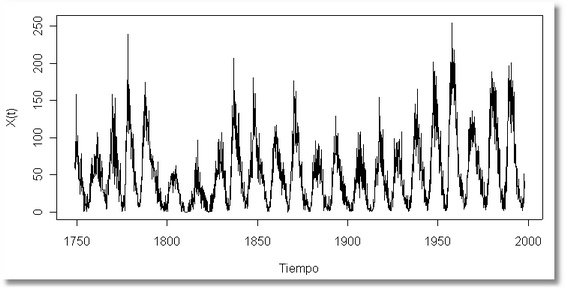
\includegraphics[width=10cm]{figs/i6.png}
%\end{center}
%\caption{Serie temporal.}
%\label{fig-serie1}
%\end{figure}
%
%El siguiente paso consistir'a en determinar si la secuencia de valores es completamente aleatoria o si, por el contrario, se puede encontrar alg'un patr'on a lo largo del tiempo, pues s'olo en este caso podremos seguir con el an'alisis.
%
%La metodolog'aa tradicional para el estudio de series temporales es bastante sencilla de comprender, y fundamentalmente se basa en descomponer las series en varias partes: tendencia, variaci'on estacional o peri'odica, y otras fluctuaciones irregulares.
%
%\paragraph{Tendencia.} Es la direcci'on general de la variable en el periodo de observaci'on, es decir, el cambio a largo plazo de la media de la serie. 
%
%\paragraph{Estacionalidad.} Corresponde a fluctuaciones peri'odicas de la variable, en periodos relativamente cortos de tiempo. 
%
%\paragraph{Otras fluctuaciones irregulares.} Despu'es de extraer de la serie la tendencia y variaciones c'iclicas, nos quedar'a una serie de valores residuales, que pueden ser o no totalmente aleatorios. Volvemos a estar como en el punto de partida, pues ahora tambi'en nos interesa determinar si esa secuencia temporal de valores residuales puede o no ser considerada como aleatoria pura.
%
%En la figura \ref{fig-serie2} vemos un ejemplo de una serie temporal en la que se aprecia la existencia de las distintas componentes comentadas
%\begin{figure}[h!]
%\begin{center}
%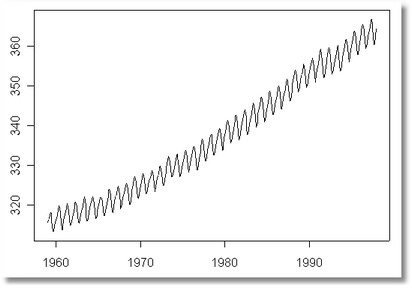
\includegraphics[width=8cm]{figs/i7.png}
%\end{center}
%\caption{Tendencia, estacionalidad y fluctuaciones irregulares.}
%\label{fig-serie2}
%\end{figure}
%
%\section{Componentes de una serie: tendencia, estacionalidad y ruido}
%
%\section{an'alisis de la tendencia}
%Una primera idea sobre la presencia de tendencia en la serie la obtendremos en su representaci'on gr'afica. Pero no siempre estar'a tan clara como en la figura \ref{fig-serie2}. Por ejemplo, en los datos de la figura \ref{fig-serie3} sigue habiendo tendencia, pero ya no es tan marcada.
%\begin{figure}[h!]
%\begin{center}
%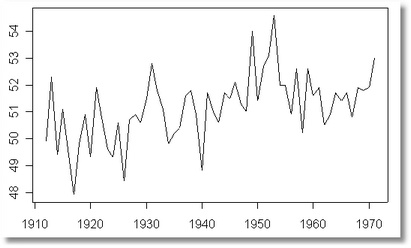
\includegraphics[width=8cm]{figs/i8.png}
%\end{center}
%\caption{Tendencia, estacionalidad y fluctuaciones irregulares.}
%\label{fig-serie3}
%\end{figure}
%
%Los medios m'as utilizados para detectar y eliminar la \textbf{tendencia} de una serie se basan en la aplicaci'on de \textbf{filtros} a los datos. Un filtro no es m'as que una funci'on matem'atica que aplicada a los valores de la serie produce una nueva serie con unas caracter'isticas determinadas. Entre esos filtros encontramos las \textbf{medias m'oviles}. 
%
%Una media m'ovil se calcula, para cada punto, como un promedio del mismo n'umero de valores a cada lado de ese punto. as'i una media m'ovil de tres puntos se calcula como:
%\begin{equation}
%m(x_t)=\frac{x_{t-1}+x_t+x_{t+1}}{3}.
%\end{equation}
%Mientras que una media m'ovil de cuatro puntos viene dada por
%\begin{equation}
%m(x_t)=\frac{x_{t-2}/2+x_{t-1}+x_t+x_{t+1}+x_{t+2}/2}{4}.
%\end{equation}
%
%Cuando la cantidad de puntos de la media m'ovil es par, se toma la mitad de los valores extremos.
%
%Existen otros procedimientos para extraer la tendencia, como \textbf{ajuste de polinomios}, entre otros. 
%
%Una clase de filtro, que es particularmente 'util para eliminar la tendencia, se basa en aplicar \textbf{diferencias} a la serie hasta convertirla en estacionaria. Una diferencia de primer orden se obtiene restando dos valores contiguos:
%\begin{equation}
%\Delta x_{t+1}:=x_{t+1}-x_t.
%\end{equation}
%Si volvemos a diferenciar esa serie, restando los nuevos valores consecutivos obtenemos una nueva serie m'as suavizada.
%\begin{equation}
%\Delta^2 x_{t+2}:=\Delta x_{t+2}-\Delta x_{t+1}.
%\end{equation}
%
%Una vez que se aplica un proceso cl'asico de descomposici'on mediante un procedimiento de medias m'oviles a los datos de la figura \ref{fig-serie2}, se obtiene las siguientes series:
%\begin{figure}[h!]
%\begin{center}
%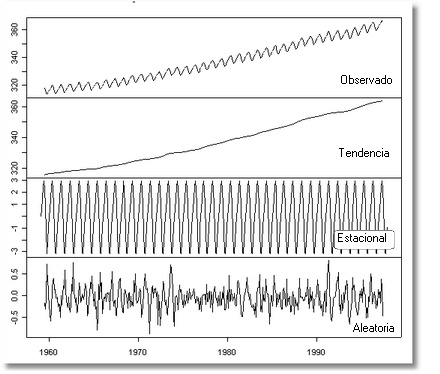
\includegraphics[width=8cm]{figs/i10.png}
%\end{center}
%\caption{Observado, tendencia, estacional, aleatoria.}
%\label{fig-serie4}
%\end{figure}
%
%Para analizar la \textbf{estacionalidad} de una serie introduciremos un concepto de gran inter'es en el an'alisis de series temporales: la \textbf{funci'on de autocorrelaci'on}. 
%
%La \textbf{funci'on de autocorrelaci'on} mide la correlaci'on entre los valores de la serie distanciados un lapso de tiempo $k$.
%
%La f'ormula del coeficiente de correlaci'on simple, dados $N$ pares de observaciones $y$, $x$:
%\begin{equation}
%r:=\frac{\sum (y_i-\bar{y})(x_i-\bar{x})}{\sqrt{\sum(y_i-\bar{y})^2\sum(x_i-\bar{x})^2}}.
%\end{equation}
%
%De igual forma, dada una secuencia temporal de $N$ observaciones $x_1,\cdots,x_N$, podemos formar $N-1$ parejas de observaciones contiguas $(x_1, x_2), (x_2,x_3),\cdots (x_{N-1},x_N)$ y calcular el coeficiente de correlaci'on de estas parejas. 
%
%A este coeficiente lo denominaremos \textbf{coeficiente de autocorrelaci'on} de orden 1 y lo denotamos como $r1$. An'alogamente se pueden formar parejas con puntos separados por una distancia $2$, es decir $(x_1,x_3), (x_2,x_4)$,  etc. y calcular el nuevo coeficiente de autocorrelaci'on de orden 2. De forma general, si preparamos parejas con puntos separados una distancia $k$, calcularemos el coeficiente de autocorrelaci'on de orden $k$.
%
%Al igual que para el coeficiente de correlaci'on lineal simple, se puede calcular un error est'andar y por tanto un intervalo de confianza para el coeficiente de autocorrelaci'on.
%
%La \textbf{funci'on de autocorrelaci'on} es el conjunto de coeficientes de autocorrelaci'on $rk$ desde 1 hasta un m'aximo que no puede exceder la mitad de los valores observados, y es de gran importancia para estudiar la estacionalidad de la serie, ya que si 'esta existe, los valores separados entre s'i por intervalos iguales al periodo estacional deben estar correlacionados de alguna forma. Es decir que el coeficiente de autocorrelaci'on para un retardo igual al periodo estacional debe ser significativamente diferente de 0.
%
%\section{m'etodos de an'alisis de componentes}
